\subsection{Applications of Basic Methods}\label{applicationsofbasicmethods}

\subsubsection{Inclusion-Exclusion}\label{inclusionexclusion}

\begin{theorem}[Inclusin-exclusion principle]
Let $A_1,A_2,\dots,A_n$ be finite sets. Then\dots
$$|A_1 \cup A_2 \dots \cup A_n| = \sum^n_{j=1}(-1)^{j-1} \sum_{i_1,i_2,\dots,i_j}|A_{i_1}\cap A_{i_2}\cap \dots \cap A_{i_j},$$
where $(i_1,i_2, \dots ,i_j)$ ranges all $j$-element subsets of $[n]$.
\end{theorem}

\begin{proof}
We prove the two follwoing claims:
\begin{enumerate}
  \item If $x$ is contained in the set represented on the left side of the equation, then the right side conts it exactly once.
  \item If $x$ is not contained in any $A_i$, then the right-hand side counts $x$ zero times.
\end{enumerate}
(1) Assume that $x$ is contained in exactly $k$ of the $n$ $A_i$-sets, with $k > 0$. Certainly, $x$ is not in any $j$-fold intersection
where $j>k$. On the otherhand $j \leq k$, then $x$ is contained in exactly ${k \choose j}$ different $j$-fold intersections. If we take
the signs into accoount, this means that the right side counts $x$ exactly\dots
$$m = \sum^k_{j=1} (-1)^{j-1} {k \choose j}$$
times. Now we show that $m=1$ necessarily. Observe\dots
$$1-m=\sum^k_{j=0}(-1)^j {k \choose j} = (1-1)^k = 0,$$
since $k$ is positive.

(2) We repeat the above argument with $k=0$. Then the \hyperref[binomialtheorem]{binomial theorem} technique we use above
gives us $(1-1)^0 = 1$, implying $m=0$.\newline

Thus the left-hand side and the right-hand side count the same objects.
\end{proof}

\subsubsection{Multisets}\label{multisets}

Given a set $A$, a \emph{multiset} is defined via a function $m : A \rightarrow \mathbb{N} \cup \{ 0 \}$. It is a set containing $a \in A$ $m(a)$ many times.

\subsubsubsection{Multinomial Coefficients}

\begin{theorem}
Given a multiset $A$ of $n$ elements over a $k$ element sets. The number of ways to linearly order the elements of $A$ is\dots
$${n \choose a_1,a_2,\dots,a_k} = \frac{n!}{a_1!a_2!\dots a_k!}.$$
\end{theorem}

\subsubsection{Weak Compositions}\label{weakcompositions}

Let $a_1,a_2,\dots,a_k$ be nonnegative integers satisfying
$$\sum^k_{i=1} a_i = n.$$
Then the ordered $k$-tuple $(a_1,a_2,\dots,a_k)$ is called a \emph{weak composition} of $n$ into $k$ parts.

\begin{theorem}
The number of weak compositions of $n$ into $k$ parts is\dots
$${n + k - 1 \choose n} = {n + k - 1 \choose k - 1}.$$
\end{theorem}

\begin{corollary}
The number of $n$-element multisets over a $k$-elemnt set is\dots
$${n + k - 1 \choose n} = {n + k - 1 \choose k - 1}.$$
\end{corollary}

\subsubsection{Compositions}\label{compositions}

Let $a_1,a_2,\dots,a_k$ be positive integers satisfying
$$\sum^k_{i=1} a_i = n.$$
Then the ordered $k$-tuple $(a_1,a_2,\dots,a_k)$ is called a \emph{composition} of $n$ into $k$ parts.

\begin{corollary}
The number of compositions of $n$ into $k$ parts is\dots
$${n - 1 \choose k - 1}.$$
\end{corollary}

\subsubsection{Stirling numbers of the second kind}\label{secondstirlingnumbers}

Given a finite set $A$, $|A| = n$, the number of set partitions of $A$ into $0 < k \leq n$ classes is denoted $S(n,k)$, the \emph{Stirling number of the second kind}.

\begin{theorem}
For all positive integers $n$ and $k$ satisfying $n \leq k$, the equality\dots
$$S(n,k) = S(n-1,k-1) + kS(n-1,k)$$
\end{theorem}

\begin{theorem}
For all positive integers $n$ and $k$ satisfying $n \geq k$.
$$S(n+1,k) = \sum_{i=0}^n {n \choose i} S(n-i, k-1)$$
\end{theorem}

\begin{theorem}
The number of \hyperref[surjection]{surjections} from $[n]$ to $[k]$ is equal to
$$\sum^k_{j=0} (-1)^j {k \choose j} (k-j)^n.$$
\end{theorem}

\begin{corollary}
For all positive integers $k \leq n,$
$$S(n,k) = \frac{1}{k!}\sum^k_{j=0} (-1)^j {k \choose j} (k-j)^n.$$
\end{corollary}

\subsubsubsection{Bell numbers}\label{bellnumbers}
The number of all partitions of a finite set $A$, where $|A| = n$, is denoted $B(n)$ and is called a \emph{Bell number}.

\begin{theorem}
Set $B(0) = 1$. Then, for all positive integers $n$,
$$B(n+1)=\sum_{k=0}^n B(k) {n \choose k}.$$
\end{theorem}

\subsubsection{Partitions of integers}\label{integerpartitions}

A \emph{partition of an integer} $n$ is a finite sequence $(a_1, a_2,\dots,a_k)$ of positive integers satisfying $a_1 \geq a_2 \geq \cdots \geq a_k$ and $a_1 + a_2 + \cdot + a_k = n$.

\begin{theorem}
As $n \rightarrow \infty$, the function $p(n)$ satisfies\dots
$$p(n)\sim\frac{1}{4\sqrt{3}}\exp{\left(\pi\sqrt{\frac{2n}{3}}\right)}$$
\end{theorem}

\subsubsection{Ferrers shapes}\label{ferrers}

The \emph{Ferrers shape} of the partition $(a_1,a_2,\dots,a_k)$ is a row diagram of squares, with non-increasing amounts of squares in lower rows. For example the Ferrers shape fo $(5,3,2)$ is\dots\newline

\begin{center}
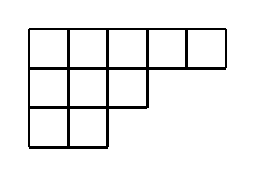
\begin{tikzpicture}[scale=0.5, line width=1pt]
  \draw (0,0) grid (5,1);
  \draw (0,0) grid (3,-1);
  \draw (0,-1) grid (2,-2);
\end{tikzpicture}
\end{center}

\begin{proposition}
For all positive integers $k \leq n$, the number of partitions of $n$ that have at least $k$ parts is equal to the number
of partitions of $n$ in which the largest part is at least $k$.
\end{proposition}

\begin{proposition}
For every positive integer $n$, the number of partitions of $n$ in which the first two parts are equal is equal to the number of partitions of $n$ 
in which each part is at least $2$.
\end{proposition}

\begin{lemma}
Let $m > k \geq 1$. Let $S$ be the set of partitions of $n$ into $m$ parts, the smallest of which is equal to $k$, and let $T$ be the set of partitions of 
$n$ into $m-1$ parts, in which the $k$th part is larger than the $(k+1)$st part and the smallest part is at least $k$.
Then $|S| = |T|$.
\end{lemma}

\subsubsection{Euler's totient function}\label{combinatoricstotient}

For any positive integer $n$, let $\phi(n)$ denote the number of positive integers $k \leq n$ that are relatively prime to $n$.

\begin{proposition}
Let $n = pq$, where $p$ and $q$ are distinct prinmes. Then $\phi(n) = (p-1)(q-1).$
\end{proposition}

\begin{proof}
Use the \hyperref[inclusionexclusion]{inclusion-exclusion principle} on $[pq]$, followed by the \hyperref[subtraction]{subtraction principle}.
\end{proof}

\begin{proposition}
Let $n = p_1p_2\dots p_t$, where the $p_i$ are pairwise distinct primes. Then\dots
$$\phi(n) = \prod^t_{i=1}(p_i - 1).$$
\end{proposition}

\begin{lemma}
Let $a$ and $b$ be two positive integers whose greates common divisor is $1$, and let $n = ab$. Then $\phi(n) = \phi(a)\phi(b).$
\end{lemma}

\begin{proposition}
For any prime $p$, and any positive integer $d$,
$$\phi(p^d) = (p-1)p^{d-1}.$$
\end{proposition}

\begin{proposition}
Let $n = p_1^{d_1}p_2^{d_2}\dots p_t^{d_t}$, where the $p_i$ are distinct primes. Then\dots
$$\phi(n) = \prod^t_{i=1}p_i^{d_i-1}(p_i - 1)$$
\end{proposition}
